\documentclass[12pt,a4paper]{article}
\usepackage[utf8]{inputenc}
\usepackage{graphicx}
\usepackage{geometry}
\usepackage{float}
\usepackage{hyperref}

\geometry{a4paper, margin=1in}

\title{\textbf{Laporan Tugas Kecerdasan Buatan}\\ \Large Natural Language Processing (NLP) - Analisis Sentimen}
\author{
    \textbf{Nama: Fransiscus Asisi Kananda Herdion Dharmawan} \\
    \textbf{NIM: 24.83.1107} \\
    \textbf{Jurusan: Teknik Komputer} \\
    \textbf{Universitas Amikom Yogyakarta}
}
\date{\today}

\begin{document}

\maketitle

\section{Pendahuluan}
Tugas ini berfokus pada implementasi algoritma \textit{Natural Language Processing} (NLP) untuk menganalisis sentimen dari dataset ulasan pengguna aplikasi di Google Play Store. Tujuan utamanya adalah untuk mengklasifikasikan teks ulasan pengguna menjadi sentimen positif atau negatif menggunakan model pembelajaran mesin.

\section{Metode}
Algoritma yang digunakan dalam eksperimen ini adalah \textbf{Support Vector Machine (SVM)} dengan kernel linear. Proses ekstraksi fitur dilakukan menggunakan \textbf{TF-IDF} (\textit{Term Frequency-Inverse Document Frequency}) dengan membatasi maksimum fitur sebanyak 5000 kata.

Adapun tahapan pra-pemrosesan (\textit{preprocessing}) yang dilakukan meliputi:
\begin{enumerate}
    \item Membersihkan baris data yang kosong (\textit{missing values}).
    \item Mengategorikan skor 1-2 sebagai \textbf{Negatif}, skor 4-5 sebagai \textbf{Positif}.
    \item Menghapus ulasan berskor 3 (\textbf{Netral}) guna memfokuskan model pada klasifikasi biner (\textit{Binary Classification}).
\end{enumerate}
Setelah proses \textit{preprocessing}, data dibagi menjadi data latih (\textit{training set}) sebesar 80\% dan data uji (\textit{testing set}) sebesar 20\%.

\section{Hasil dan Pembahasan}

Distribusi sentimen pada dataset yang telah disaring dapat dilihat pada Gambar \ref{fig:distribusi}. Kelas Positif cenderung lebih banyak daripada kelas Negatif.

\begin{figure}[H]
    \centering
    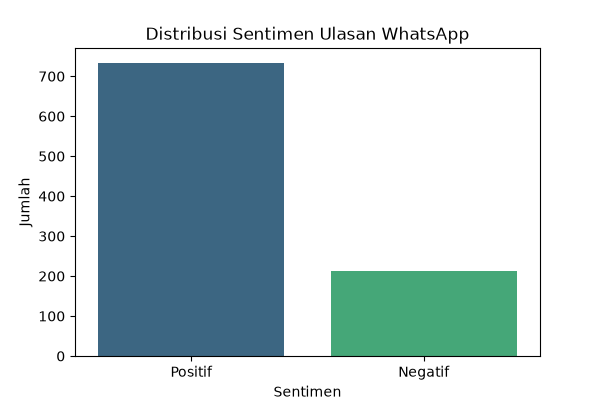
\includegraphics[width=0.7\textwidth]{sentiment_distribution.png}
    \caption{Distribusi Sentimen Ulasan WhatsApp}
    \label{fig:distribusi}
\end{figure}

Setelah dilakukan proses pelatihan (\textit{training}), model dievaluasi pada data uji (\textit{testing set}). Model Support Vector Machine menghasilkan metrik performa sebagai berikut:
\begin{itemize}
    \item \textbf{Akurasi}: 88.95\%
    \item \textbf{Precision}: 92.00\%
    \item \textbf{Recall}: 95.00\%
    \item \textbf{F1-Score}: 93.00\%
\end{itemize}

Hasil matriks kebingungan (\textit{Confusion Matrix}) dari prediksi model dapat dilihat pada Gambar \ref{fig:cm}.

\begin{figure}[H]
    \centering
    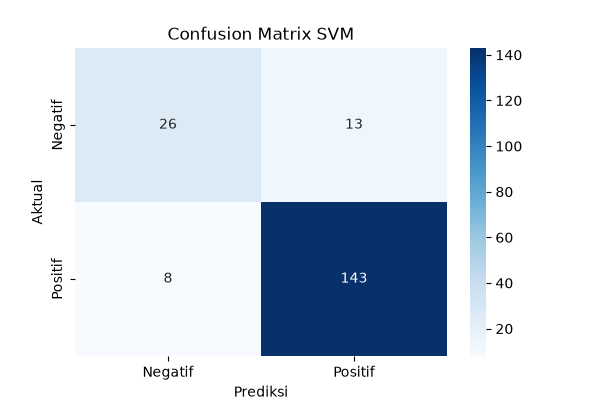
\includegraphics[width=0.7\textwidth]{confusion_matrix.png}
    \caption{Confusion Matrix Model SVM}
    \label{fig:cm}
\end{figure}

\section{Kesimpulan}
Berdasarkan hasil evaluasi, model \textit{Support Vector Machine} (SVM) dengan ekstraksi fitur TF-IDF mampu mengklasifikasikan sentimen ulasan secara sangat baik dengan tingkat akurasi mencapai sekitar 88.95\% dan \textit{F1-Score} untuk kelas positif mencapai 93.00\%. Hal ini menunjukkan bahwa algoritma SVM sangat cocok dan tangguh untuk digunakan pada kasus analisis teks dan NLP.

\section*{Tautan Pengujian}
Seluruh kode \textit{Jupyter Notebook} untuk pra-pemrosesan data, pelatihan model, dan evaluasi hasil secara langsung dapat diakses dan dijalankan melalui tautan Google Colab berikut: \\
\url{https://colab.research.google.com/drive/1Hvsv7HF6zmiZhnLucfXnqz0VO0ycthnq?usp=sharing}

\end{document}
